\documentclass {article}
\usepackage{graphicx}
\usepackage{amsmath}
\begin{document}

\title{How to Structure a LaTeX Document}
\author{Andrew Roberts}
\date{December 2004}
\maketitle

Dear Eric,

Easiest for me to write this paper to you. It makes the audience easy to visualize and I have an idea about your level of mathematical/physics sophistication. Before I get into it, I want to remind you that I do have a master’s degree in Physics from the CUNY education system, where I took essentially every graduate class that they offered.

Tell me where I lose you. What I really hope is that I don’t lose you in the assumptions. The point is to take some simple assumptions and see if they lead to something interesting.

I’d also like to thank you for reading this. It makes for an audience, where I don’t have to present my findings in a way consistent with Physics research papers that are published, but I can hopefully talk in a more casual manner while keeping the math rigorous.


\section{Introduction}
This section's content...
	Hello World!
$$	\pi^2 = \frac 1 2 $$
Normal text is easy to write?

\subsection{Two Paradigms}
In the early 20th century, Einstein started two revolutions in theoretical physics. The first is the theory of general relativity. The other based on an explanation of the photoelectric effect and the need to quantized radiation culminated in quantum mechanics after decades of work from many researchers. 

General relativity is a theory of gravity and spacetime. It made three bold claims: precession , etc.

Quantum mechanics is a strange theory for those uninitiated (and still strange even to them). At the heart of the standard model is the Dirac equation. The Dirac equation is the awesomest.

\subsection{The need for Quantum Gravity}

Thus our current state of physics has two competing paradigms in physics, on the large-scale is General Relativity, and on the opposite spectrum is quantum mechanics. These are paradigms are like water and oil, and a successful mixture of the two has not been accomplished. “The mind calls for a third theory to unify all of physics, and for a simple reason. Nature is in an obvious sense “unified.” The universe we find ourselves in is interconnected, in that everything interacts with everything else. There is no way we can have two theories of nature covering different phenomena, as if one had nothing to do with the other. Any claim for a final theory must be a complete theory of nature.” (underline mine, because I make no claim that this is a final theory) “The intellect seeking after an integrated theory cannot rest content with the assumption that there exist two distinct fields totally independent of each other by their nature,” Einstein said in his Nobel lecture in 1923.

“Besides the argument based on the unity of nature, there are problems specific to each theory that call for unification with the other. Each has a problem of infinities. In nature, we have yet to encounter anything measurable that has an infinite value. But in both quantum theory and general relativity, we encounter predictions of physically sensible quantities becoming infinite. This is likely the way that nature punishes impudent theorists who dare to break her unity.”

“General relativity has a problem with infinities because inside a black hole the density of matter and the strength of the gravitational field quickly become infinite… 

In quantum theory, “Quantum theory gives only statistical predictions of subatomic behavior. Our ability to do any better than that is limited by the uncertainty principle, which tells us that we cannot measure a particle’s position and momentum at the same time.” <- otherwise you get an infinity, there are uncontrollable fluctuations in the values of every quantum variable. Look at the zpr”  

“There has long been the hope that when gravity is taken into account, the fluctuations will be tamed and all will be finite. If infinities are signs of missing unification, a unified theory will have none. It will be what we call a finite theory, a theory that answers every question in terms of sensible, finite numbers.”

In addition, he believed there was a link between the need to resolve apparent paradoxes of quantum mechanics and the need to unify electromagnetism and gravity. Einstein always insisted that quantum mechanics could be derived from some more complete theory. For Einstein, who was never satisfied with the weirdness and randomness inherent in quantum theory, any acceptable unified field theory had to have quantum mechanics as a consequence.” (https://www.aps.org/publications/apsnews/200512/history.cfm)

\subsection{Other proposals}
	

“Over the last three decades, theorists have proposed at least a dozen new approaches. Each approach is motivated by a compelling hypothesis, but none has so far succeeded. In the realm of particle physics, these include Technicolor, preon models, and supersymmetry. In the realm of spacetime, they include twister theory, causal sets, supergravity, dynamical triangulations, and loop quantum gravity. Some of these ideas are as exotic as they sound.
	
	“One theory has attracted more attention than all the others combined: string theory.”  a theory in which point-like particles are replaced by strings that vibrate in various ways. On distance scales larger than the string scale, a string looks just like an ordinary particle, with its mass, charge, and other properties determined by the vibrational state of the string[1]. 
	
	“Part of the reason string theory makes no new predictions is that it appears to come in an infinite number of versions… With such a vast number of theories, there is little hope that we can identify an outcome of an experiment that would not be encompassed by one of them. Thus, no matter what the experiments show, string theory cannot be disproved. But the reverse also holds: No experiment will ever be able to prove it true.” 
	
	“In science, for a theory to be believed, it must make a new prediction -- different from those made by previous theories -- for an experiment not yet done. For the experiment to be meaningful, we must be able to get an answer that disagrees with that prediction. When this is the case, we say that a theory is falsifiable -- vulnerable to being shown false. The theory also has to be confirmable; it must be possible to verify a new prediction that only this theory makes. Only when a theory has been tested and the results agree with the theory do we advance the theory to the ranks of true theories.”
	
	However string theory has failed… or it might be even easier to say it is such a failure that it cannot even fail, because in its current state it is not even testable. A physical theory that is not testable is hard to disprove. But even more importantly, 50 years without any tangible results might give anyone pause. Here are two quotes summarizing the current state of string theory:
	
	Brian Green Quote [The fabric of the cosmos (2004)]: “Even today, more than three decades after its initial articulation, most string practitioners believe we still don’t have a comprehensive answer to the rudimentary question, What is string theory? … [M]ost researchers feel that our current formulation of string theory still lacks the kind of core principle we find at the heart of other major advances.”
	
	David Gross, a Nobel laureate … and a formidable champion of string theory, … “We don’t know what we are talking about… The state of physics today is like it was when we were mystified by radioactivity… They were missing something fundamental. We are missing perhaps something as profound as they were back then.”
	
	\subsection{A new theory}
		I believe a fresh approach is warranted, especially since we know that string theory has hit a wall, and after close to 50 years a new approach is warranted.
		
		This paper attempts to show what is missing. Rather than trying to combine general relativity with quantum mechanics, it seems possible that one of the two (or even both) is wrong. I believe that general relativity is wrong. What I present in this paper is a new theory of gravity.
		
		Is it very new? Not really, it is based on solid math that was present over a hundred years ago. Many people were on a similar arc at the turn of the last century, however Einstein up-ended that and work in this direction stopped.
		
		What would a new theory of gravity look like? It would need to cover all the basics of Newtonian Gravity and General Relativity. It should also offer something testable to tell the two apart.
		
		Finite theory, the infinities should disappear.
		
		Obey the uncertainty principle, “Quantum theory gives only statistical predictions of subatomic behavior. Our ability to do any better than that is limited by the uncertainty principle, which tells us that we cannot measure a particle’s position and momentum at the same time.”
		
		In addition, he believed there was a link between the need to resolve apparent paradoxes of quantum mechanics and the need to unify electromagnetism and gravity. Einstein always insisted that quantum mechanics could be derived from some more complete theory. For Einstein, who was never satisfied with the weirdness and randomness inherent in quantum theory, any acceptable unified field theory had to have quantum mechanics as a consequence.” (https://www.aps.org/publications/apsnews/200512/history.cfm)
		
		Anything else? Yes, a theory should hopefully not only explain the facts and offer testable differences, but it should also in some way offer enlightenment, beauty and a clearer understanding of the universe. 
		
\subsection{My Theory: Maxwell's equations  + ZPR}

All good theories should start with an insight that is hopefully clean, transparent and maybe even obvious. Mine is that gravity and radiation should be treated as “duals” of each other.

As I will show in section 2.5, the Maxwell equations naturally divide into two sets of equations: one governing radiation and the other governing gravity. 

I believe that we should use the Maxwell equations as the fundamental equations of gravity and radiation. As if gravity and radiation were two sides of the same coin. 

I propose that the attraction of mass to mass known as "gravity" can be explained, not by the bending of space-time, as in Einstein's theory of General Relativity, but by incorporating the background radiation of the universe into Maxwell's equations of electromagnetism.

\subsection{Plan of the Paper}
Plan of the Paper

Much of the work in this paper, because I am trying to re-do gravity is focused on showing that my theory can both accomplish the equations that Newton left us, i.e., Newton’s equation of gravity for a mass in its rest-frame. I then set out to show that my theory can also get the same results that Einstein showed with his theory, namely the precession of the perihelion of mercury, the red-shift/blue-shift of light as it falls down a gravity well, and finally the ending of light around a massive object. I will also point out a few places where testable differences are perhaps possible.

Finally, I look at how this theory of gravity would fit in with quantum mechanics. I do this by deriving from only the equations that I had already developed in previous parts of the paper the Dirac equation. Afterwards, probably in an appendix, I then use the dirac equation to derive some of the celebrated results of quantum mechanics.

\section{Assumptions}
	
	As I will explain, there are several facts of the universe and several true assumptions of this theory. But I wanted to put them all in one section, because they are the building blocks of this theory. The facts of the universe are zero point radiation and Heisenberg’s uncertainty principle. We will also take a page from General Relativity in taking the idea that a black hole has an event horizon after which we can no longer know what happens within a massive object.
	
\subsection{Cosmic Microwave Background Radiation}


Hey, it’s a fact of the universe. But necessary for me to put in the assumption category. 

Most importantly we have the zero-point energy. 

We should also mention that we need to keep things stochastic, but that they generally don’t interact in the approximate to anything that one would not expect.

\subsection{Maxwell’s Equations}

They’re awesome!


\subsection{Massive Atom}

The distribution of the mass will fortunately be something we can side-step as I will show in the Radius cut-out section.

\subsection{Massive Atom with Temperature}

Hey, it’s a fact of the universe. But necessary for me to put in the assumption category. 

Even the core of the moon is hot enough to melt rock. Scientists believe that the outer core of the moon is still molten lava. This may be obvious, but it is nice to understand that gravity creates a pressure, which means that even rock will melt for something as small as the moon. And it is one of the assumptions of this paper (and really an experimental fact) that all massive particles have a temperature. What does this mean precisely at a quantum level? Well it is a fact that even as you approach absolute zero on the Kelvin scale, all particles will still vibrate (provable by Heisenberg’s uncertainty principle). It is this vibration that I call and most people would agree as having temperature.

Finally though, what we are interested in is a small massive particle. Where does it get its energy so that it does not collapse. The assumption we make is that it absorbs energy from the zero point radiation. 

\subsection{Radius cut-out}

Maybe this is really the biggest assumption, se we have to show some particular historical material. Because one of the assumptions is that the surface of the mass is in some type of quantum boil, the surface doesn’t need to be constant. We want to create a shell far away from the quantum boil. We cannot ignore quantum fluctuations and we assume that we can mimic the quantum behavior and say that it is stochastic behaviour. Is that reasonable?

Too help out with our understanding, we should first like to show that without anything extra, a massive particle will collapse under its own weight. Therefore, we will need an extra term to balance out this collapse. This really might belong in the main section better, but I guess it really is an assumption… Or maybe I have to put it after declaring the Maxwell equations…. 

Two infinities are present in the physics: one term from the equations of gravity and one term from the equations of radiation. Both infinities can be dealt with by a simple trick: cutting off a sphere surrounding the particle/atom in its system of rest. The radius of this cutoff is related to both the event-horizon and the Hawking radiation of a black hole.

It’s also possible way above here and talk about gravity and radiation in the same breadth. Then ...

I’ll get to the equations in a bit, but first I’d like to discuss the philosophical implications of this. First of all, is it reasonable? The answer is yes. In General Relativity, the event-horizon is where General Relativity breaks down, so we are not subtracting from any knowledge gained from using General Relativity. We are in fact cutting off our theory at the same point and declaring anything smaller a no-man’s land. On the other hand, in terms of quantum mechanics, A cut-off is frequently introduced for the exact same reasons (to quell the infinities) and we are again not subtracting from the knowledge of quantum mechanics. Secondly, it also seems reasonable in terms of Heisenberg’s uncertainty principle. We know that if we wish to become too precise when looking at the position of a particle, the momentum (i.e., it’s radiation) goes to infinity, and on the other hand when we are too precise in looking at the momentum, then the position of the particle becomes unknown. In fact a gaussian distribution gives us the best accuracy we can do for both, exactly solving the heisenberg uncertainty principle. Here is the math for that:

What we show next is that we can use several similar distributions of mass to gain an understanding of how they work in concert:

\subsubsection{Spherical shell}

\subsubsection{Solid sphere}

As I’ve shown, all these different distributions give the same result up to a factor of one. The truth is, and I probably should have mentioned this up higher, is that many of these equations were tried over a hundred years ago when devising a theory of the electron. In the case of classical electron theory, because all the solutions were equivalent up to a factor of one, this was chosen as the classical radius of an electron. We will follow suit and declare a similar radius for a massive atom.

An immediate consequence of this choice, leaves us with several startling implications: We notice that this cutoff gives us the same radius as that described by General Relativity for a blackhole, and also implies the exact radiation spectrum cutoff as that implied by Hawking Radiation.

And as mentioned in the section Massive Atom, we have shown how we side-step the issue of the distribution of mass.

\subsection{Conclusion of the Assumptions}

I believe that if you have made it through all of these assumptions, then the rest of the paper will be straight-forward mathematical applications and that I’ve already won if you have made it this far.


\section{Section 1}

Postulate 1: We assume that gravity is correctly described by Maxwell's Equations:

$$\nabla \times \vec B  - \partial_t \vec E  = -4 \pi G \vec J ~~~~~~~~ \nabla \times \vec E + \partial_t \vec B = 0    ~~~~~~~~~~~ (1)$$

$$\nabla \cdot \vec E = -4 \pi G \rho ~~~~~~~~~~ \nabla \cdot \vec B = 0   ~~~~~~~~~~~ (2)$$

and, for completeness, the conservation of mass-charge:

$$\nabla \cdot \vec J + \partial_t \rho = 0 ~~~~~~~~~~~ (3)$$

Where we are in units where c = 1. The constant G differs in different systems of units. In SI units, it is equal to $6.674 \times 10^{-11} \frac {N \cdot m^2}{kg^2}$ .

\subsection{Celestial Mechanics}

Skipping this sub-section is totally okay, but for completeness and as a way to introduce some notation, let's actually go ahead and derive that the gravitational field follows the inverse square law. 

For a static mass distribution, we have:

$$\rho = m \delta^3_x  ~~~~~~~~~~~ (4)$$

where I am purposefully being a little bit non-commital about the delta function. In this present paper, it doesn't matter so much, but I think it's best to leave it a little open for future work. With that said, we can still say that outside of some radius R, it looks like a pure delta function... i.e.,

$$\delta^3_x = \delta(\vec x) ~~~ \textrm{if} ~~~ r > R ~~~~~~~~~~~ (5)$$

Hopefully, it is not surprising, that we can then write the "static Gravitational field" like:

$$\vec{E}_I(\vec x) = -G \int \rho(\vec x') \frac {\vec x - \vec x'}{|\vec x - \vec x'|^3} d^3x ~~~~~~~~~~~ (6)$$

This immediately implies (see the text and equations around Jackson 1.14):

$$\nabla \cdot \vec{E}_I = -4 \pi G \rho ~~~~~~~~~~ \nabla \times \vec{E}_I = 0 ~~~~~~~~~~~ (7)$$

Following Berrara [link](http://iopscience.iop.org/article/10.1088/0143-0807/6/4/014/meta) we assume that any vector field, $\vec V$, and any scalar, $g$, can be expanded as follows:

$$\vec V (\vec x) = \sum_{l=0}^{\infty} \sum_{m=-l}^{l} \left[a_{lm}(r) \vec Y_{lm}(\theta, \phi) +b_{lm}(r) \hat r \times \vec X_{lm} (\theta, \phi) +c_{lm}(r) \vec X_{lm} (\theta, \phi) \right] ~~~~~~~~~~~ (8)$$

$$g(\vec x) = \sum_{l=0}^{\infty} \sum_{m=-l}^{l} g_{lm}(r) Y_{lm}(\theta, \phi) ~~~~~~~~~~~ (9)$$

where $Y_{lm}$ are the usual spherical harmonics (see Jackson 3.53), $\vec Y_{lm}$ is simply $\hat r Y_{lm}$  and $\vec X_{lm}$ is defined as,

$$\vec X_{lm}(\theta, \phi) = \frac {-i}{\sqrt{l(l+1)}} \vec r \times \left( \nabla Y_{lm}(\theta, \phi) \right) ~~~~~~~~~~~ (10)$$

Using these definitions and after some slightly painful algebra, we can write out the final solution:

$$\vec E_I(\vec x) = \sum_{l,m} \left[ -\frac {4\pi i G }{2l+1} \frac {q_{lm}}{r^{l+2}} \sqrt {l(l+1)} \left(\hat r \times \vec X_{lm} \right)  - \frac {4 \pi G (l+1)}{2l+1} \frac {q_{lm}}{r^{l+2}} \vec Y_{lm} \right] ~~~~~~~~~~~ (11)$$

where

$$q_{lm} \equiv \int Y_{lm}^* (\theta, \phi) r^l \rho (\vec x ) d^3x = \int \rho_{lm} (r) r^{l+2}dr ~~~~~~~~~~~ (12)$$

Clearly then, if

$$\rho = m\delta(\vec x) ~~~~~~~~~~~ (13)$$

We get

$$\vec E_I(\vec x) = - \frac {mG} {r^2}  ~~~~~~~~~~~ \textrm{if} ~~~ r > R ~~~~~~~~~~~ (14)$$

as expected.

\subsection{Precession of the Perihelion of Mercury}

For moving distributions, we need to take into account that a gravitational-magnetic field is introduced via

$$\vec B = \vec \beta \times \vec E ~~~~~~~~~~~ (15)$$

See the text around Jackson 11.150 for more information. 

Using the small-velocity approximation 

$$\vec B \approx \vec v \times \vec E ~~~~~~~~~~~ (16)$$

we can find the same equations as Einstein used to describe the precession of the perihelion of Mercury's orbit. I have worked this out, but apparently I am not the first to do so, please see [link](https://www.researchgate.net/publication/226889193\_Gravitomagnetism\_A\_novel\_explanation\_of\_the\_precession\_of\_planets\_and\_binary\_pulsars) and/or [link](https://arxiv.org/pdf/gr-qc/0311030.pdf) . (I can certainly supply my own derivation of these results, but it might take me a week or two to go back over my own work and make it understandable.)

To be precise, according to Sean M. Carroll's book "An Introduction to General Relativity: Spacetime and Geometry", we can write:

$$\frac 1 2 \left( \frac {dr}{d\lambda} \right)^2 + V(r) = \mathcal{E} ~~~~~~~~ \textrm{(Carrol 5.65)} ~~~~~~~~~~~ (17)$$

where

$$V(r) = \frac 1 2 \epsilon - \epsilon \frac {GM} r + \frac {L^2}{2r^2} - \frac {GML^2}{r^3} ~~~~~~~~ \textrm{(Carrol 5.66)} ~~~~~~~~~~~ (18)$$

According to Carroll: "A similar analysis of orbits in Newtonian gravity would have produced a similar result; the general equation (5.65) would have been the same, but the effective potential (5.66) would not have had the last term. (Note that this equation is not a power series in $1/r$, it is exact.)"

However, in our present theory, not only can we derive the last term (the term proprtional to $1/r^3$), but we see that this is only the low-limit approximation. I am not an experimentalist, but I believe that this would be a ripe area to explore whether this theory can produce results more accurate than General Relativity.


\subsection{Solenoidal and Irrotational Form of Maxwell's Equation}

In the first draft of this paper, I didn't include this section because I thought it would be an extra step that was basically unnecessary. While this is true, and all of the results in the rest of the paper can still be derived, it actually tends to make the math a little cleaner to split the Maxwell equations into their Irrotational and Solenoidal forms.

A vector $\vec V$ can be split into a solenoidal vector $\vec V_S$ and an irrotational vector $\vec V_I$:

$$\vec V = \vec V_I + \vec V_S ~~~~~~~~~~~ (19)$$

where

$$\nabla \cdot \vec V_S = 0 ~~~~~ \nabla \times \vec V_I = 0 ~~~~~~~~~~~ (20)$$

Using this notation we can rewrite the Maxwell equations into irrotational equations:

$$\nabla \cdot \vec E_I = -4 \pi G  \rho ~~~~~~~~~~~ (21)$$

$$\nabla \cdot \vec J_I + \partial_t \rho = 0 ~~~~~~~~~~~ (22)$$

$$ \partial_t \vec E_I = 4 \pi G \vec J_I ~~~~~~~~~~~ (23)$$

And solenoidal equations:

$$\nabla \times \vec E_S + \partial_t \vec B_S = 0 ~~~~~~~~~~~ (24)$$

$$\nabla \times \vec B_S - \partial_t \vec E_S =  - 4 \pi G \vec J_S ~~~~~~~~~~~ (25)$$

The thing we really want to say, and I'm not sure if this is an assumption or is just totally obvious, is that, at least when we are in the rest frame of the mass (which is the frame of reference that we will be in for the rest of this paper), these equations de-couple. We have one set of equations that describe the forces due to the mass and another set of equations that describe radiation. We can make this explicit by defining a new current:

$$\vec {J_S'} = - G \vec {J_S} ~~~~~~~~~~~ (26)$$

which changes the inhomogenous Solenoidal equation into:

$$\nabla \times \vec B_S - \partial_t \vec E_S =  4 \pi \vec {J_S'} ~~~~~~~~~~~ (27)$$

but affects none of the other equations at all!

Because this form of the equations is the same as that presented in books on radiation. I will get rid of the prime on the Solenoidal current, and use the following equations as the solenoidal (radiation) Maxwell equations:

$$\nabla \times \vec B_S - \partial_t \vec E_S =  4 \pi \vec J_S ~~~~~~~~~~~ (28)$$

$$\nabla \times \vec E_S + \partial_t \vec B_S = 0 ~~~~~~~~~~~ (29)$$

When this difference in constant impacts the equations that follow, I will note the difference, so please don't think I am trying to pull a fast one here.

\section{Section 2}

This section concerns the two classical test of General Relativity concerning the bending of light around a massive object and the blue-shift of light as it falls down towards a massive object.

Postulate 2: Empty space is filled with a randomly-fluctuating zero-point energy and a massive object absorbs some of this energy, thereby preventing collapse of the mass. I therefore postulate that a massive object induces a “field” (or maybe a momentum-flow is a better way to say it?) in the surrounding space and when a photon travels through this “field,” the momentum of the photon is shifted in an additive and linear manner – in accordance with the following equation: 

$$\Delta \vec p = \int_{path} \vec P ~ dl ~~~~~~~~~~~ (30)$$

where we integrate along the path of the photon and $\vec P$ is defined as

$$\vec P = - \hat r \frac {Gm\hbar}{r^2} ~~~~~~~~~~~ (31)$$

\subsection{Bending of light}

We imagine a photon that emanates from a distant source, passes close by a massive object, then continues beyond the object to an observer. The closest point while passing, i.e., the impact parameter, is at a distance of $b$ from the center of the object. For ease of calculation, we will say that both the point of emanation and the observer are infinitely far from the massive object.

\begin{center}
	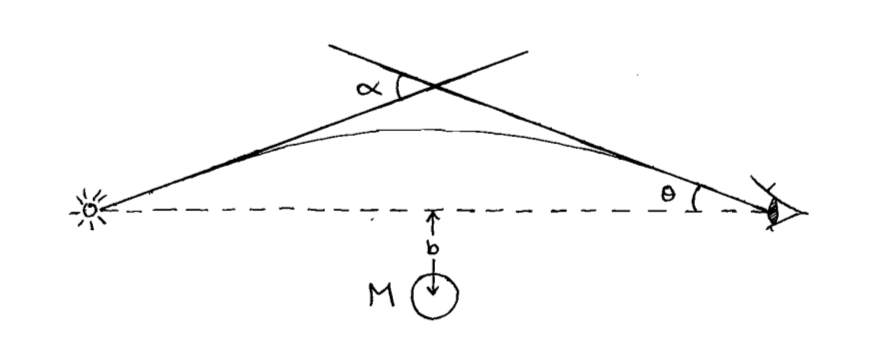
\includegraphics[scale=0.4]{light-bending.png}
\end{center}


We assume that to a first-order approximation the trajectory of the photon is a straight line. To calculate its change in momentum, we integrate along the straight-line path of the photon:

$$\Delta \vec p = \int_{path} \vec P ~ dl = \int_{-\infty}^{\infty} - \frac {Gm\hbar}{r^3} \vec r ~ wdz ~~~~~~~~~~~ (32)$$

We divide the problem into two parts: the momentum change in the direction parallel to the direction of travel of the photon and the momentum change perpendicular to the direction of travel. In calculating the momentum change in the direction parallel to the direction of travel, we note that as the photon approaches and then recedes from the massive object, the change in momentum cancels out to leave zero net change in the parallel direction. We can easily calculate the change in momentum in the direction perpendicular to the direction of travel:

$$\Delta p_y = \int_{-\infty}^{\infty}  \frac {Gm\hbar}{(z^2 + b^2)^{3/2}} b ~ wdz ~~~~~~~~~~~ (33)$$

This yields:

$$\Delta p_y = \hbar w \frac {2Gm} b ~~~~~~~~~~~ (34)$$

We therefore get:

$$\theta \approx \sin \theta = \frac {\Delta p_y}{p_z} = \frac {2Gm} b ~~~~~~~~~~~ (35)$$

Which yields the deflection angle:

$$\alpha = \frac {4Gm} b ~~~~~~~~~~~ (36)$$

This is the same result as in the theory of General Relativity.

\subsection{Blue-shift of light }

Using the same postulate, we can calculate the blue-shift of light. As a photon falls into a gravity well, the momentum and hence the energy of the photon are shifted. Because the energy of a photon is generally expressed as a frequency, we say that the frequency of the photon observed at infinity is changed compared to when it is observed in a gravitational field at a distance R from the center of the massive object. We use the following equation to express this change:

$$\hbar w' = \hbar w + \Delta p ~~~~~~~~~~~ (37)$$

To calculate the change in momentum, we again integrate along the path of the photon:

$$\Delta p = \int_{\infty}^R \hat r \cdot \vec P w dr= \int_{\infty}^R - \frac {Gm\hbar}{r^2} w dr = \hbar w \frac {Gm}R ~~~~~~~~~~~ (38)$$

This yields:

$$\hbar w' = \hbar w \left( 1 + \frac {Gm}R \right) ~~~~~~~~~~~ (39)$$

In the theory of General Relativity the equation is given as: 

$$\hbar w ' = \hbar w (1 - 2Gm/R)^{-1/2} ~~~~~~~~~~~ (40)$$

As Gm/R approaches zero, my equation and the equation from General Relativity converge.  As Gm/R approaches one, however, the equations diverge.  This could be another testable difference between my theory and Einstein's.

\subsection{Backwards derivation of my postulate}

The only equation necessary from this analysis, is the one that is boxed, near the end of this section. Otherwise this section can be skipped, but I think it is worth talking a bit more about my postulate, on a mathematical level. 

Since we are talking about radiation, we use the Solenoidal Maxwell equations and write the general solution in free-space as:

$$\vec E_{S}(\vec x, w,l,m) = \frac i {k} a_E M_1(w,l,m) \nabla \times \left(f_l(kr) \vec X_{lm} \right) + a_M M_2(w,l,m) f_l(kr) \vec X_{lm} ~~~~~~~~~~~ (41)$$

$$\vec B_{S}(\vec x, w,l,m) =  a_E M_1(w,l,m) f_l(kr) \vec X_{lm} - \frac i {k} a_M M_2(w,l,m) \nabla \times \left(f_l(kr) \vec X_{lm} \right) ~~~~~~~~~~~ (42)$$

See Jackson 9.122 for details.

Where we have introduced $M_{\lambda}(w,l,m)$ to indicate that the radiation is stochastic, where:
\begin{equation}
\left< M_{\lambda}(w,l,m) \right> = 0 ~~~~~~~~~~~ (43)
\end{equation}

$$\left< M_{\lambda}(w,l,m)M_{\lambda'}^*(w',l',m') \right> = \delta_{\lambda \lambda'} \delta_{ll'}\delta_{mm'}\delta(w - w') ~~~~~~~~~~~ (44)$$ 

Philosophically, this makes a lot of sense to me. However, if we are willing to take the time-average of the physical quantities of interest, we do not need these Stochastic terms at all. 

Using either a time-average (and a temporary integration over angles) or using this Stochastic method gives:

\begin{multline}
$$\left< \vec E_S \times \vec B_S^* \right> = \sum_{l,m} \int dw ~ \frac i k \left[ |a_E|^2\left( \nabla \times \left( f_l(kr) \vec X_{lm} \right)\right) \times \left(f^*_l(kr) \vec X_{lm}^* \right) \right.
\\ \left.- |a_M|^2 \left( f^*_l(kr) \vec X_{lm}^*\right) \times \left( \nabla \times \left( f_l(kr) \vec X_{lm}\right)\right)\right] ~~~~~~~~~~~ (45)$$
\end{multline}


Because we are looking for answers that are electromagnetically neutral, we require that $|a_E|^2 = |a_M|^2$. Using the Wronskian, see Jackson 9.91, and assuming incoming waves, leaves:

$$\left< \vec E_S \times \vec B_S^* \right> =  - 2 \sum_{l,m} \int dw \frac {|a_E|^2}{k^2 r^2} | \vec X_{lm} |^2 \hat r ~~~~~~~~~~~ (46)$$

In the electromagnetic units that we are working in, momentum is defined as:

$$\vec P = \frac 1 {8 \pi} \int d^3x \left< \vec E_S \times \vec B_S^* \right> ~~~~~~~~~~~ (47)$$

Therefore,

$$\vec P = - \frac {\hat r} {4 \pi} \int d^3x \int dw \frac 1 {k^2 r^2} \sum |a_E|^2 |\vec X|^2 ~~~~~~~~~~~ (48)$$

To me, my postulate at the beginning of this section is the same as taking 

$$\sum |a_E|^2 |\vec X|^2 = \frac 2 {\pi} Gm \hbar k^4 ~~~~~~~~~~~ (49)$$

This yields:

$$\boxed{~~  \vec P = \frac 1 {(2 \pi)^3} \int d^3x \int d^3k \left(- \hat r \frac {Gm \hbar} {r^2}\right) ~~ } ~~~~~~~~~~~ (50)$$

If we had instead worked in Gravitational units, we would have had

$$\vec P = - \frac 1 {8 \pi G} \int d^3x \left< \vec E_S \times \vec B_S^* \right> ~~~~~~~~~~~ (51)$$

which would have changed the postulate of $|a_E|^2$, and would have required outgoing waves instead ... 

\section{Section 3}

In this section we will derive an equation that is very reminiscent of the Dirac equation.

Postulate 3 Ohm's law:

$$\vec J_S = \sigma \vec E_S  ~ \delta^3_x \delta^3_k ~~~~~~~~~~~ (52)$$

where $\delta^3_x$ keeps the current on the surface of the mass, and $\delta^3_k$ relates the allowed frequencies to the radius of the mass. 

As mentioned in section 1, I feel comfortable stating that outside of some radius R, the delta function in x reduces to the normal point delta function. However, the delta function over k is given here with a quite abnormal normalization. I require that

$$\frac 1 {(2 \pi)^3} \int \delta^3_k d^3k = 1 ~~~~~~~~~~~ (53)$$

... I know that this is weird. Let me try to motivate it a little. If we take the combination of the two, we get:

$$\frac 1 {(2 \pi)^3} \int d^3x \int d^3k ~ \delta^3_k \delta^3_x = 1 ~~~~~~~~~~~ (54)$$

Looking back at the boxed equation above, what I am basically suggesting is that many of the equations of interest generally exist under this type of double integration, and we essentially take this "density" as the quantity of interest. Essentially, this is a way for us to keep the quantities of interest "On Shell".

In the end, I believe I am allowed to take my postulates how I see fit and in the following calculation, we will not really need to be any more specific about these delta functions. 

\subsection{Calculate $\sigma$ By Saying That a Mass Doesn't Implodes}

To calculate $\sigma$, we use Equation (6.114) from Jackson:

$$\int \left[ \rho \vec E_I +  \frac 1 2 \vec J_S \times \vec B_S^* \right]d^3x = 0 ~~~~~~~~~~~ (55)$$

Taking into account that the radiation has random fluctuations (or, similarly, we can take the time-average), we have:

$$\int \left[ \rho \vec E_I +  \frac 1 2 \left< \vec J_S \times \vec B_S^* \right> \right]d^3x = 0 ~~~~~~~~~~~ (56)$$

This is the equation that we need to ensure that the zero-point energy is supplying enough energy so that the mass does not implode.

Let's deal with the two terms seperately:

$$\int \rho \vec E_I d^3x = -\hat r \int \frac {Gm^2}{r^2} \delta^3_x d^3x ~~~~~~~~~~~ (57)$$

Using our postulate that 

$$\frac 1 {(2 \pi)^3} \int \delta^3_k d^3k = 1 ~~~~~~~~~~~ (58)$$

we can write the above as

$$\int \rho \vec E_I d^3x = -\frac {\hat r}{(2 \pi)^3} \int \frac {Gm^2}{r^2} \delta^3_x  \delta^3_k d^3x d^3k ~~~~~~~~~~~ (59)$$

Turning our attention to the second term:

$$\int d^3x \frac 1 2 \left< \vec J_S \times \vec B_S^* \right>  = \sigma \int d^3x \delta^3_x \delta^3_k \frac 1 2 \left< \vec E_S \times \vec B_S^* \right>  ~~~~~~~~~~~ (60)$$

Using the boxed equation from section 2, we have

$$\int d^3x \frac 1 2 \left< \vec J_S \times \vec B_S^* \right> = -\hat{r} \frac 1 {(2 \pi)^3} \int d^3x \int d^3k \frac {4\pi G m\hbar}{r^2} \sigma ~~~~~~~~~~~ (61)$$

therefore, in order for these two terms to equal out, we require:

$$\sigma = - \frac m {4 \pi \hbar} ~~~~~~~~~~~ (62)$$

If instead of using the usual electromagnetic radiation constants, we had used the Gravitational constants, we would have found:

$$\sigma =  \frac m {4\pi G \hbar} ~~~~~~~~~~~ (63)$$

\subsection{Deriving the Dirac Equation}

Either using the electromagnetic radiation constants or the Gravational constants allows us to rewrite Maxwell's  current equation as:

$$\nabla \times \vec B_S  - \partial_t \vec E_S  = - \frac m {\hbar} \vec E_S ~~ \delta^3_x \delta^3_k ~~~~~~~~~~~ (64)$$

If we promise to only work "On shell", we can therefore write this as

$$\nabla \times \vec B_S  - \partial_t \vec E_S  = - \frac m {\hbar} \vec E_S ~~~~~~~~~~~ (65)$$

Using the dual transform, see Jackson 6.150, we can re-write the two Solenoidal equations:

$$-\partial_t \vec E_S + \nabla \times \vec B_S   +\frac m {\hbar} \vec E_S = 0 ~~~~~~~~~~~ (66)$$ 

$$ -\partial_t \vec B_S - \nabla \times \vec E_S   +\frac m {\hbar} \vec B_S = 0 ~~~~~~~~~~~ (67)$$ 

We also note that we can write:

$$\nabla \times \vec V = g_i \partial_i \vec V ~~~~~~~~~~~ (68)$$

where the $g_i$s are defined:

$$g_1 = \left(\begin{matrix}  0 && 0 && 0 \\ 0 && 0 && -1 \\ 0 && 1 && 0 \end{matrix}\right) ~~~~~~~~~~~ (69)$$

$$g_2 = \left(\begin{matrix}  0 && 0 && 1 \\ 0 && 0 && 0 \\ -1 && 0 && 0 \end{matrix}\right) ~~~~~~~~~~~ (70)$$

$$g_3 = \left(\begin{matrix}  0 && -1 && 0 \\ 1 && 0 && 0 \\ 0 && 0 && 0 \end{matrix}\right) ~~~~~~~~~~~ (71)$$

we therefore re-write Maxwell's equations as 

$$-\partial_t \vec E_S + g_i \partial_i \vec B_S   +\frac m {\hbar} \vec E_S = 0 ~~~~~~~~~~~ (72)$$ 

$$ -\partial_t \vec B_S - g_i \partial_i \vec E_S   +\frac m {\hbar} \vec B_S = 0 ~~~~~~~~~~~ (73)$$ 

if we the define 

$$\psi = \left(\begin{matrix}  \vec E_S \\ \vec B_S \end{matrix}\right) ~~~~~~~~~~~ (74)$$

and 

$$\gamma^0 = \left(\begin{matrix}  -1 && 0 \\ 0 && -1 \end{matrix}\right) ~~~~~~~~~~~ (75)$$

$$\gamma^i = \left(\begin{matrix}  0 && g_i \\ -g_i && 0 \end{matrix}\right) ~~~~~~~~~~~ (76)$$

We can again re-write Maxwell's equations as

$$\left(\gamma^{\mu} \partial_{\mu} + \frac m {\hbar} \right) \psi = 0 ~~~~~~~~~~~ (77)$$

which can be compared with, for example, Sakurai's book "Advanced Quantum Mechanics" equation 3.31.

As I mentioned in the email. This is not the Dirac Equation because these gamma matrices do not transform correctly.


\end{document}